\section{User Testing} \label{sec:s4_test}
%%% Intro paragraph

In order to evaluate the usefulness of the crowd condition visualisation from the previous section, we conducted a user test\sinote{Is this a good term?}. In this section we will describe the test and analyse its results.

\subsection{Test Method}

In order to measure the performance of the system, we ask the test subject to analyse a test data scenario, that contains some interesting crowd condition situations. If the system visualises the crowd conditions in a good way, The test subject would be able to understand the crowd conditions.

We start the test with a very simple \enquote{tutorial}. Its purpose is to give the test subject an intuition of how the density, velocity and turbulence overlays behave and the information they can provide. \Cref{fig:tutorial_screens} provides a visual illustration of this. Since the pressure condition would require a more thorough explanation not suitable for this short test, we will not evaluate the pressure overlay in the test.

\sinote{Annoter alle figurer og brug disse annoteringer til forklaringer}

\begin{figure}[htbp]
\begin{subfigure}[t]{.49\linewidth}
    \centering
    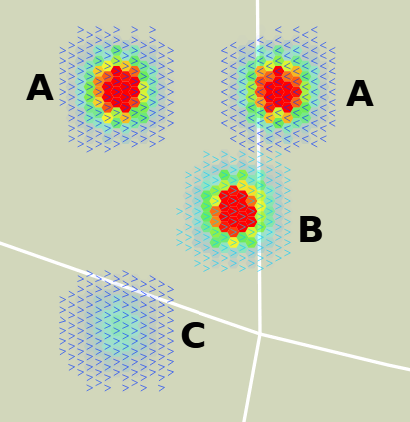
\includegraphics[width=\linewidth]{velocity_density_tutorial.png}
    \caption{Velocity and density - Groups A and B The top three groups are all more dense than the bottom group. The third group from the top moves at a faster rate than the rest.}
\end{subfigure}
\enspace
\begin{subfigure}[t]{.49\linewidth}
    \centering
    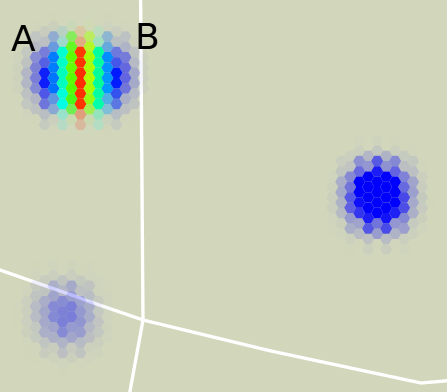
\includegraphics[width=\linewidth]{turbulence_tutorial.png}
    \caption{Turbulence - The top two groups are \enquote{crashing} which shows up as high turbulence.}
\end{subfigure}
\caption{Screenshots of the tutorial scenario}
\label{fig:tutorial_screens}
\end{figure}

\sinote{oddly shaped infinity sign - nej, brug annoteringer}

After the tutorial scenario, we will switch to a more detailed data set. The data set is artificially created by us, and resembles a normal day on SmukFest with a variety of interesting situations. \Cref{fig:test_data_screens} shows this visualised. A large, dense crowd is standing in front of a stage. South of the stage, people are moving in an oddly shaped infinity sign. This means that there is a crossroad, where groups of people are meeting. In the top left corner of the area, people are moving in opposite directions close to each other. 

\begin{figure}[htbp]
\begin{subfigure}[t]{.49\linewidth}
    \centering
    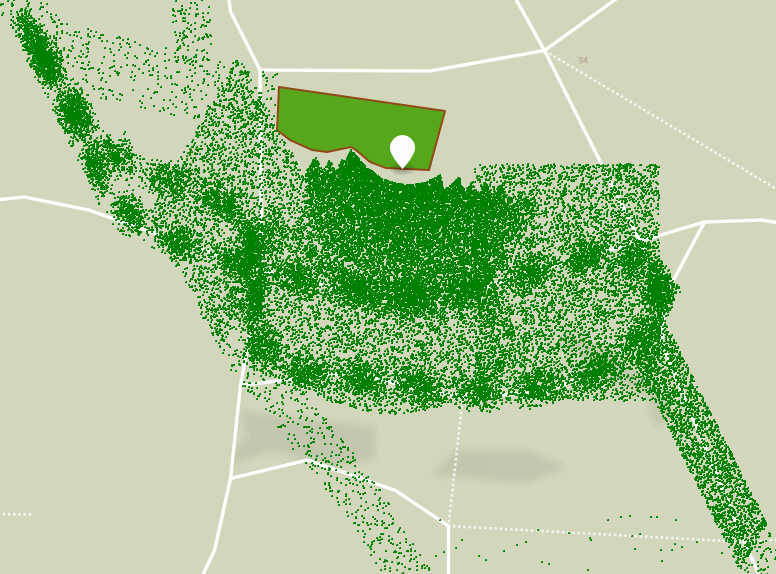
\includegraphics[width=\linewidth]{people_test_data.png}
    \caption{Distribution of people - Each green dot represents a person.}
\end{subfigure}
\enspace
\begin{subfigure}[t]{.49\linewidth}
    \centering
    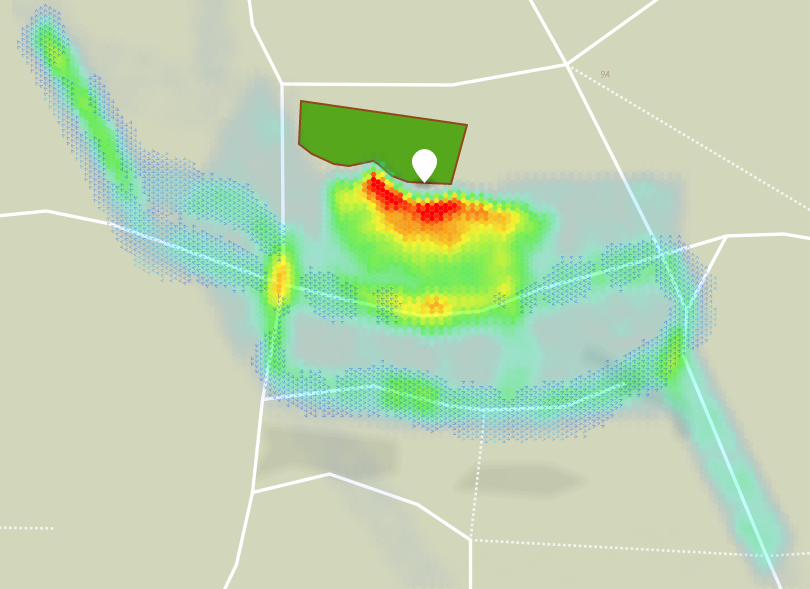
\includegraphics[width=\linewidth]{velocity_density_test_data.png}
    \caption{Velocity and density - The crowd is very dense at center stage and also at a few positions where multiple groups of people meet. Velocity can be seen at the oddly shaped infinity sign south of the stage.}
\end{subfigure}
\enspace
\begin{subfigure}[t]{.49\linewidth}
    \centering
    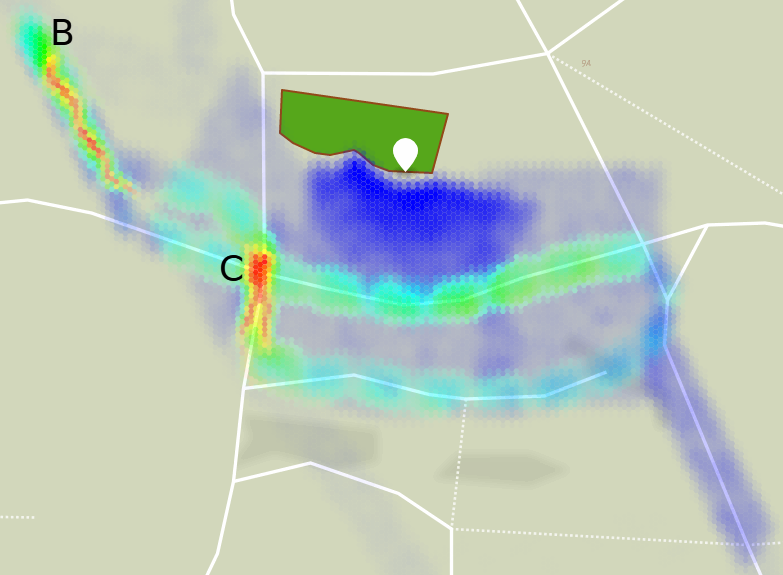
\includegraphics[width=\linewidth]{turbulence_test_data.png}
    \caption{Turbulence - The turbulence is high at two positions; at the crossroads of the oddly shaped infinity sign and at the very top left corner. Even though density at center stage is high, the turbulence is low. This indicates that people are standing close to each other, but there is little movement. This would indicate that the high density area in front of the stage is less of a threat.}
\end{subfigure}
\caption{Screenshots of the test data scenario}
\label{fig:test_data_screens}
\end{figure}

Anders Nord of Alarm HS, kindly agreed to participate in this user test. The user test was performed over Skype as in other meetings. Anders was presented with the application which was configured to display the aforementioned predefined crowd scenarios. 

%%% Testing results, high abstraction level
\subsection{Test Results}
\sinote{Vi kan måske være lidt mindre positiv her. Prøv at være mere kritisk på fejl og mangler}
Anders immediately noticed, using the density overlay, that the density was high in front of the stage, and at the crossroads where people meet. 

Switching to the velocity overlay, he did not immediately notice the arrows, as they were small. When we hinted that there were arrows, he was able to find the cycle of moving people in the oddly shaped infinite sign. Having both the velocity and density overlays enabled at the same time, Anders understood why the density was high at the crossroads; Many groups were heading to the crossroad.

The meaning of the turbulence overlay was not completely clear to Anders as he turned it on, but he quickly noticed that there was no turbulence at the area in front of the stage. His hypothesis was that the crowd was standing still at the area, which we could confirm. He also noticed the high turbulence at the crossroad and at the top left corner.

Overall, Anders was able to find all the interesting situations we had put in the test data, meaning that the visualisations of the system were good. He expressed that he was not completely confident in his knowledge about what each overlay represents. He suggested that a user of the system receives some sort of training on the system.







